\documentclass[12pt,a4paper]{article}

\usepackage{fullpage}
\usepackage[utf8]{inputenc}
\usepackage{amsfonts}
\usepackage{amssymb}
\usepackage[french]{babel}
\usepackage[cyr]{aeguill}
\usepackage{natbib}
\usepackage{graphicx}
\usepackage{tabularx}
\usepackage{hyperref}
\usepackage[document]{ragged2e}
\setlength{\parindent}{2em}
\setlength{\parskip}{1em}

\newcommand{\quotes}[1]{``#1''}

\begin{document}

\begin{titlepage}
\centering
{\scshape\LARGE Université de Bordeaux \par}
{\scshape\Large Master 1 Informatique  \par}
\vspace{3cm}

{\Huge\bfseries Projet de Programmation\par}
{\Huge\bfseries Le Clicodrome de LEFFF \par}
{\Large\bfseries par Lionel CLEMENT \par}
\vspace{0.5cm}
{\Large\itshape Mémoire \par}
{\large 05 Avril 2019\par}

\vfill
réalisé par \par
JELLITE \textsc{Oumayma} \par
BAKIR \textsc{Fatima Ezzahra} \par
NEDELEC \textsc{Guillaume} \par
SYLLA  \textsc{Alfred Aboubacar} \par
\vfill

{\large Enseignants responsables : Philippe NARBEL et Vincent PENELLE\par}

\end{titlepage}

\newpage
\tableofcontents

\newpage\section{Contexte général du projet}
\subsection{Résumé}

\smallbreak Dans ce rapport, nous avons présenté minutieusement notre étude, la conception et le développement d'un site web / Interpréteur :
    \textbf{" Le Clicodrome de LEFFF "}

Pour déterminer les formes fléchies d'un mot en français, notre client Lionel CLEMENT à donc créer un lexique "LEFFF"  contenant un grands nombre de mots de différentes catégories. Cependant, ce lexique est présenter sous format texte qui ne facilite pas l'accès, la modification et l'enrichissement du lexique.
Donc , Nous avons conçu de développer ce site web afin de faciliter l'accès au LEFFF, sa modification et son enrichissement ainsi que la génération des formes fléchies à partir d'un Interpréteur  pour  rendre ce lexique utilisable par n'importe quelle personne qui souhaiterai l'accéder.
Le présent rapport va décrire en détail, les différentes étapes suivies tout au long de ce projet allant de l'étude, 
en passant par la conception et en terminant par la réalisation de l'application.
\subsection{Présentation du projet}
\subsection{Analyse de l'existant}

\section{Analyse des besoins}
\subsection{Analyse des besoins fonctionnels}
\subsection{Analyse des besoins non fonctionnels}
\subsection{Contraintes}

\section{Architecture et description du logiciel}

\section{Analyse du fonctionnement et tests}

\section{Conclusion}
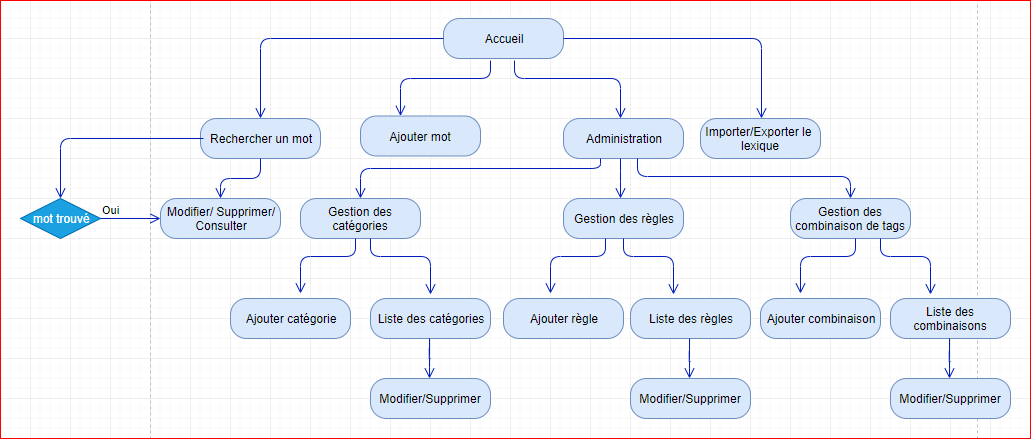
\includegraphics[width=150mm]{site.png}
\section{Références}
\bibliography{references}
\bibliographystyle{plain}
\end{document} 
